\documentclass{article}

% Packages
\usepackage{titling}
\usepackage[utf8]{inputenc}
\usepackage[english]{babel}
\usepackage{amsmath,amssymb}
\usepackage{graphicx}
\usepackage{float}
\usepackage{subcaption}
\usepackage[hidelinks]{hyperref}
\usepackage{xcolor}
\usepackage{listings}
\usepackage[a4paper, margin=1in]{geometry}
\usepackage{multicol}
\usepackage{booktabs}
\usepackage{array}

\graphicspath{{Figures/}}
\newcolumntype{M}[1]{>{\centering\arraybackslash}m{#1}}



% Title page information
\pretitle{
  \begin{center}
  \LARGE
  
\includegraphics[width=15.1cm,height=3.05cm]{Logo_unipv.png}\vspace*{1cm}\\[\bigskipamount]}


\title{\Large Machine Learning Course\vspace{0.8cm}\\
    \rule{\textwidth}{0.3pt}\vspace{0.3cm}\\
    \textbf{Movie Reviews}\vspace{0.1cm}\\
    \rule{\textwidth}{0.3pt}\vspace{0.8cm}}

\posttitle{\end{center}}
    
\author{Andrea Alberti\vspace{0.5cm}\\
    \small Department of Computer Engineering - Data Science\\[0.2cm]
    \small University of Pavia, Italy \\
    \small Email: andrea.alberti01@universitadipavia.it}\vspace{0.5cm}
        
\date{\today}

\begin{document}


\begin{titlepage}
    \maketitle
    \thispagestyle{empty}
\end{titlepage}

\tableofcontents
\thispagestyle{empty}

\newpage
\pagenumbering{arabic}



%---------------------------------------------------------

%\begin{multicols}{2}
    
\section{Introduction}
Text classification is used in many areas, such as spam filtering and document sorting. Sentiment analysis is a fascinating application that involves predicting the 
emotions of writers, such as anger, happiness, and sadness. It is useful for analyzing people's opinions on products, books, TV shows, and political parties.

\subsection{Available Data}
The dataset presented in the paper "Learning Word Vectors for Sentiment Analysis" by Andrew L. Maas et al. will be utilized. It contains 50,000 reviews that are 
equally distributed across two classes. The dataset divided into a training set of 25,000 reviews, a validation set of 12,500 reviews, and a test set of 
12,500 reviews.
\subsection{Goal}
The goal of this project is to fit a Multinomial Naive Bayes classifier to the training set and use it to predict whether a new unseen review is positive or negative.

\subsection{Naive Bayesian Classifier}
The Multinomial Naive Bayes classifier is a simple probabilistic generative classifier based on applying Bayes' theorem with strong independence assumptions between the features.
In particular the features are integers values and in this case are represented by the Bag of World representation (discussed later) of each review. Since the model is a generative
one it works by estimating the probability of each feature given the class and then using Bayes' theorem to compute the probability of the class given the feature vector.
\subsection*{Formal description}
Here is described the model in a more formal way:\\
\\
1. The goal is to find $P(Y|X)$ which is the probability of a class (Y = y) given the feature vector \\
(X = x). This is compute using Bayes' theorem.
    \vspace{0.3cm}\begin{center} $\max_y{P(Y|X)} = \frac{P(X|Y)P(Y)}{P(X)}$ \end{center}\vspace{0.3cm}

\noindent
2. Introducing the Naive independence assumption assuming $P(X|Y)$ follows a multinomial distribution where $\pi_{y,j}$ is the probability of the j-th feature given the class y 
$P(X_j|Y=y)$ and ${x_j}$ is the number of times the j-th feature appears in the document.\\
    \vspace{0.3cm}\begin{center} 
        $
        P(X|Y = y) = \frac{(x_1 + x_2 + ... + x_n)!}{x_1!x_2!...x_n!} \prod_{j=0}^{n-1} \pi_{y,j}^{x_j}
        $ \end{center}\vspace{0.3cm}

\noindent
3. Inserting 2 inside 1 and applying logarithm we obtain:
    \vspace{0.3cm}\begin{center} ${P(Y = y|X)} = \sum_{j=0}^{n-1} x_j \log{\pi_{y,j}} + \log{P(Y)}$ \end{center}\vspace{0cm}
    \begin{center} and \end{center}\vspace{0cm}
    \begin{center} $\hat{y} = arg\max_y {P(Y = y|X)} = \sum_{j=0}^{n-1} x_j \log{\pi_{y,j}} + \log{P(Y)}$ \end{center}\vspace{0.3cm}

\noindent
Basically we classify to the class (Y = y) maximizing the function in point 3. The parameters of the model are the $\pi_{y,j}$ and the $P(Y)$ which are estimated simply
computing the relative frequencies of the features and the classes in the training set. For example:

    \vspace{0.3cm}\begin{center} $\pi_{y,j} = \frac{N_{X_j, Y=y}}{N_{Y=y}}$ \end{center}\vspace{0.3cm}



%-----------------------------------------------------------

\section{Model Building}
To use the Multinomial Bayesian Classifier for text classification it is necessary to perform 3 steps. First of all a vocabulary containing the words that will be used
to represent the reviews must be built. Then the features must be extracted from the reviews, creating the BoW representation of each review. Finally the classifier 
must be trained.

\subsection{Build a vocabulary}
The vocabulary is built taking the most frequent words in the training set. Since the number of words taken can influence the performance of the model, the vocabulary
size is varied in the "Changing Vocabulary Size" section and the results are compared. The vocabulary is created in the following way:\\
\\
1. The training set is read and the words are tokenized removing punctuation, capital letters and words shorter than 3 characters.\\
\\
2. The words are counted and the most frequent ones are taken and stored in a txt file.


\subsection{Extract Features}
The features are extracted from the reviews creating the Bag of Words representation. The features are the words in the vocabulary and the value of each feature is the
number of times the word appears in the review.

\subsection{Train Classifier}
The training phase is just the application of what said in the "Formal description" section. Using the relative frequencies the parameters to learn are:\\
\\
1. The probability distribution of each word inside each class $\pi_{y,j}$.\\
\\
2. The probability distribution for the class $P(Y = y)$.\\
\\
\textbf{Model performance}\\
A first result of the train and test accuracies of the model, together with some specifications are reported in table \ref{tab:base_model}:

    \begin{table}[H]
        \centering
        \caption{\small Base Model performance}
        \label{tab:base_model}
        \begin{tabular}{|c|c|c|c|c|}
        \hline
        \textbf{Version} & \textbf{Training set} & \textbf{Vocabulary size} & \textbf{Train accuracy} & \textbf{test accuracy}\\
        \hline
        Base & Full & 1000 & 0.820 & 0.816\\
        \hline
        \end{tabular}
    \end{table}

\noindent
The model has already a good performance since the accuracy is above 80\%. In particular the model is neither overfitting nor underfitting since the train and test accuracy are
quite similar. However the model can be improved and in the next section some variants are proposed.\\
\subsection{Variants}
The variants proposed are two:\\
\\
1. Try to exclude a list of the most common words in the English language.\\
2. Use the stemming technic to make the model to not distinguish among words with the same root.\\
\\
\textbf{Excluding common words}\\
To add this modification to the base version we need first of all to have a list of the words we want to exclude. The list is in the file \textit{'stopwords.txt'}.
A new vocabulary excluding the words in this latter is created and its size can be freely chose. At this
point the BoW must be adapted to the new vocabulary and all is set. The model can now be trained and tested.\\
\\
\textbf{Introducing stemming}\\
The functions have been designed to support the optional \textit{stemming} argument. If set to \textit{True} the
functions use the Porter Stemmer algorithm to stem the words read from the files. Once again a new vocabulary is built and the BoW is adapted to the new vocabulary.\\
\\
\textbf{Comparison}\\
In the table \ref{tab:comparison_table} is reported a comparison between the base model and the two variants. A more detailed comparison is done at the end of the report, 
in the "Changing Vocabulary size" section where also the training set and  the vocabulary size are varied.

    \begin{table}[H]
        \centering
        \caption{\small Model performance comparison}
        \label{tab:comparison_table}
        \begin{tabular}{|c|c|c|c|c|}
        \hline
        \textbf{Version} & \textbf{Training set} & \textbf{Vocabulary size} & \textbf{Train accuracy} & \textbf{test accuracy}\\\hline
        Base & Full & 1000 & 0.820 & 0.816\\\hline
        Stopwords & Full & 1000 & 0.829 & 0.826\\\hline
        Stemming & Full & 1000 & 0.823 & 0.817\\\hline
        Stem + Stop & Full & 1000 & 0.826 & 0.820\\\hline
        \end{tabular}
    \end{table}

\noindent The results show that the model with the stopwords excluded performs better than both, the base model and the one with stemming with the specifications reported
in the table \ref{tab:comparison_table}. In the last row there are the results of the model with both stemming and stopwords excluded. The results are not better than
the one with the stopwords excluded.


%-----------------------------------------------------------
    
\section{Model Analysis}
In this section is done a comparison among the four models above proposed and the model with the best performance is chosen. This latter is then analyzed 
in order to understand what are the words that are more important for the model to make the classification and what are the worst error it does, in order to 
understand what are the possible improvements.

\subsection{Changing Vocabulary Size}
The vocabulary size is varied in order to see how the performance of the various models is affected. The tried sizes are five: 250, 500, 1000, 1500 and 2000 words.
The results are reported in figure \ref{fig:comparison} and figure \ref{fig:delta}.\\

    \begin{figure}[H]
        \centering
        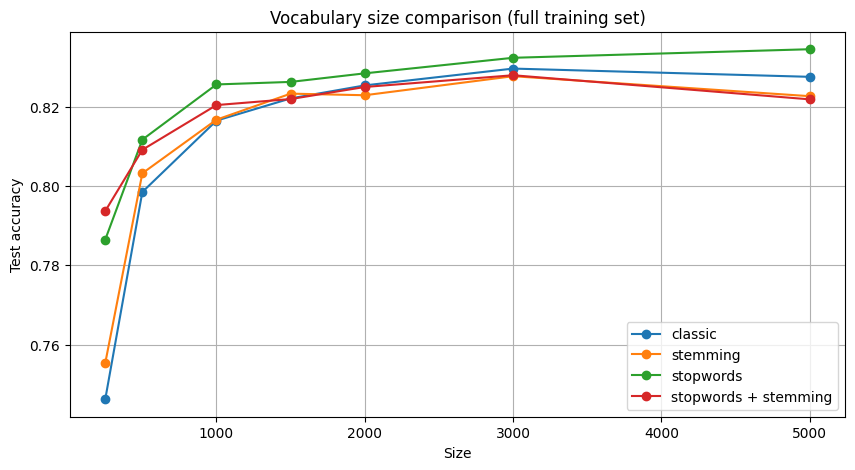
\includegraphics[width=0.8\textwidth]{vocsize_comparison_plot.png}
        \caption{\small Test accuracies comparison}
        \label{fig:comparison}
    \end{figure}

    \begin{figure}[H]
        \centering
        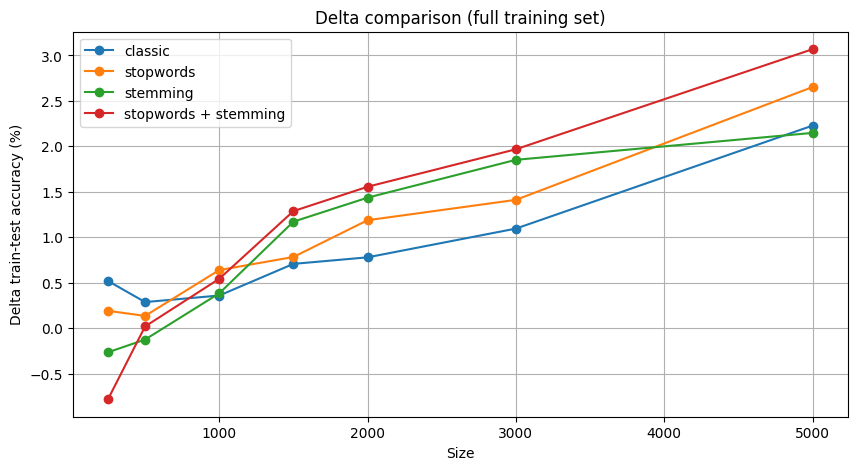
\includegraphics[width=0.8\textwidth]{delta_comparison.png}
        \caption{\small Delta error comparison}
        \label{fig:delta}
    \end{figure}

\noindent
As expected the accuracy of the model increases with the vocabulary size. However the increase is not linear and after a certain size of the vocabulary the accuracy
stays almost constant. In the figure \ref{fig:delta} is reported the delta between the training accuracy and the test accuracy as a function of the vocabulary size.
For all the model the delta increases with the growing of the vocabulary size, suggesting that the model is overfitting. This is reasonable because the number of
parameters to learn increases with the vocabulary size. Some model, like the red one are more prone to overfitting.
The model that doesn't consider stopwords is the best, probably because because it excludes the words that are most frequently used, for example the conjunction 'the'
which actually doesn't provide any information about the sentiment of the review. From now on, the model considered is the one that excludes the stopwords with a vocabulary
size of 1000 words. This is a good compromise between computational cost and model performance, since the test accuracy is high and the delta is almost the 
lowest among the models.\\


\subsection{Analysis}
\textbf{Most impactful words} varying the vocabulary size for the model.\\
The most impactful words for a class are those that most influence the classification score in favour of that class. They are taken looking at the probability
gap of each word between the two classes.
Results are reported in table \ref{tab:positive_class_impact} and table \ref{tab:negative_class_impact}.


\begin{multicols}{2}

    \begin{table}[H]
        \centering
        \caption{\small Positive Class}
        \label{tab:positive_class_impact}
        \begin{tabular}{ |c|c|c| } 
        \hline
        \textbf{Voc size} & \textbf{Word} & \textbf{Score} \\ \hline
        1000 & superb & 1.737 \\ \hline
        1000 & stewart & 1.643 \\ \hline
        1000 & wonderful & 1.586 \\ \hline
        1000 & fantastic & 1.530 \\ \hline
        1000 & excellent & 1.485 \\ \hline
        1000 & amazing & 1.415 \\ \hline
        1000 & powerful & 1.326 \\ \hline
        1000 & favorite & 1.289 \\ \hline
        1000 & perfect & 1.268 \\ \hline
        1000 & brilliant & 1.251 \\ \hline
        \end{tabular}
    \end{table}


    \begin{table}[H]
        \centering
        \caption{\small Negative Class}
        \label{tab:negative_class_impact}
        \begin{tabular}{ |c|c|c| } 
        \hline
        \textbf{Voc size} & \textbf{Word} & \textbf{Score} \\ \hline
        1000 & waste & -2.601 \\ \hline
        1000 & pointless & -2.435 \\ \hline
        1000 & worst & -2.268 \\ \hline
        1000 & awful & -2.208 \\ \hline
        1000 & poorly & -2.201 \\ \hline
        1000 & lame & -1.962 \\ \hline
        1000 & horrible & -1.891 \\ \hline
        1000 & pathetic & -1.880 \\ \hline
        1000 & wasted & -1.818 \\ \hline
        1000 & crap & -1.816 \\ \hline
        \end{tabular}
    \end{table}

\end{multicols}
\vspace{0.3cm}
\break
\noindent
\textbf{Worst errors} for the chosen model.\\
The worst errors produced by the model are the data misclassified with the higher confidence. In other words, are the reviews for which the gap between the
classification scores of the two classes is the largest. They are shown in figure \ref{fig:falsepos} and figure \ref{fig:falseneg}.

\vspace{0.3cm}
\begin{multicols}{2}

    \begin{figure}[H]
        \centering
        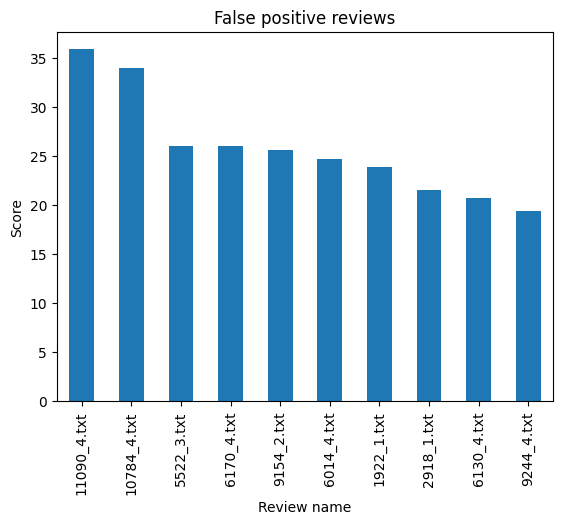
\includegraphics[width=0.44\textwidth]{false_positives.png}
        \caption{\small False positives}
        \label{fig:falsepos}
    \end{figure}

    \begin{figure}[H]
        \centering
        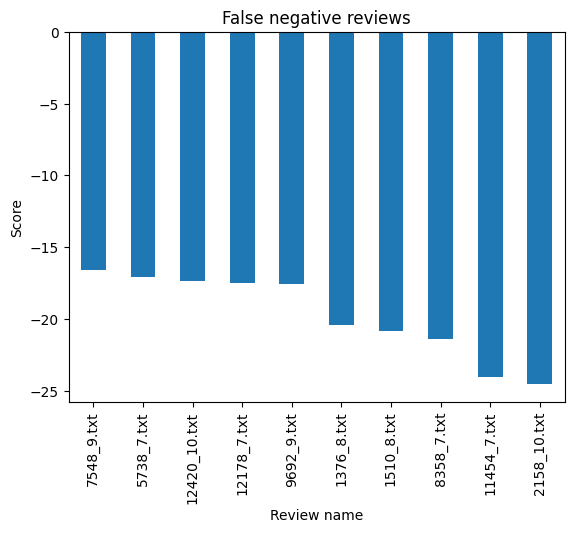
\includegraphics[width=0.44\textwidth]{false negatives.png}
        \caption{\small False negatives}
        \label{fig:falseneg}
    \end{figure}

\end{multicols}

\section{Logistic Regression}
For completeness the movie review problem is also faced using the Logistic Regression model.
\subsection{Results}
The model is a Logistic Regression without regularization, fitted on the stopwords version of the problem. The hyper parameters used together with the results are written in table \ref{tab:hyper_lr}.
In general the results are quite good similarly to the ones obtained with the Naive Bayes model.
In figure \ref{fig:falseposlr} and figure \ref{fig:falseneglr} are shown the worst errors by logistic regression. 

    \begin{table}[H]
        \centering
        \caption{\small Hyper parameters}
        \label{tab:hyper_lr}
        \begin{tabular}{ |c|c|c|c|c|c|} 
        \hline
        \textbf{N\_iter max} & \textbf{Tolerance} & \textbf{Actual N\_iter} & \textbf{Learning rate} & \textbf{train\_acc} & \textbf{test\_acc}\\ \hline
        300000 & 0.0001 & 83100 & 0.0023 & 0.867 & 0.854 \\ \hline
        \end{tabular}
    \end{table}


    \begin{multicols}{2}

        \begin{figure}[H]
            \centering
            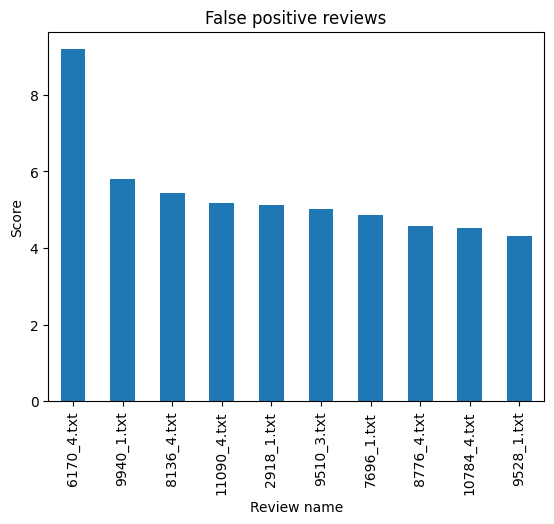
\includegraphics[width=0.44\textwidth]{false_positives_lr.png}
            \caption{\small False positives}
            \label{fig:falseposlr}
        \end{figure}
    
        \begin{figure}[H]
            \centering
            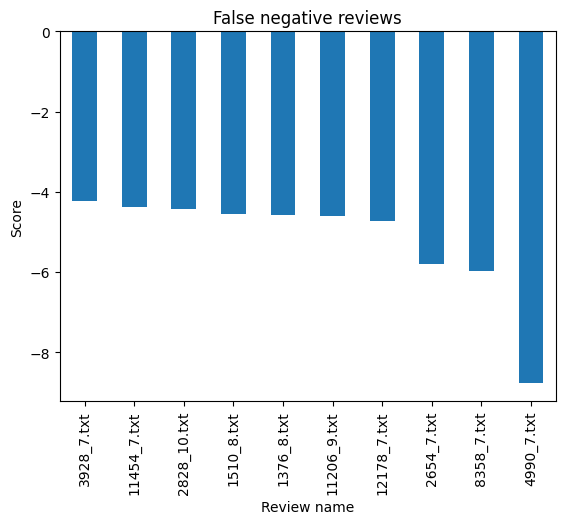
\includegraphics[width=0.44\textwidth]{false negatives_lr.png}
            \caption{\small False negatives}
            \label{fig:falseneglr}
        \end{figure}
    
    \end{multicols}


\vfill
\subsection*{\normalsize Declaration}
I affirm that this report is the result of my own work and that I did not share any part of it with anyone else except the teacher.

%\end{multicols}

\end{document}